\section{Lesson 6 ``Presentar a la gente + miembros de la famifia''}

Hi! how's it going?.\\
I'm Andy also know as ``the inglesito'' and I'm here to help you with your
English.

Soy Andy tambien conocido como ``el inglesito'' y estoy aquí para ayudarte con
tu ingles.

En esta lección aprenderas como presentar a la gente y otra justificación
para las formas largas.

Let's begin!\\
¡Empecemos!

This is my dad.\\
Este es mi Papá.

o más formalmente

Este es mi Padre.\\
This is my father.

Esta es mi mamá.\\
This is my mum.

más formalmente.\\
Esta es mi madre.\\
This is my mother.

Este es mi hermano.\\
This is my brother.

Esta es mi hermana.\\
This is my sister.

En ingles no distinguimos entre ``esta es...'' y ``este es...''

Para producir el sonido ``this'', aique morder la puntita de la lengua y
tambien el sonido se lo hace con la voz, decir como si estubiecemos
pronunciando la vocal a del español y luego morder la puntita de la lengua.

Este es Pablo.\\
This is Pablo.

Esta es Ana.\\
This is Ana.

Este es Juan. él es de españa.\\
This is Juan. He's from Spain.

Las formas acortadas son las que existen para mejorar la fluidez al hablar.

He is - He's\\
Madrid is - Madrid's\\
I am - I'm\\
You are - You're\\

En cada caso es más fácil contraerlo.

\begin{figure}[H]
\centering
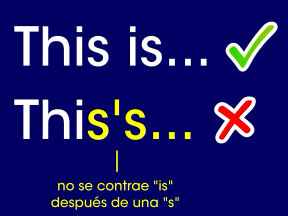
\includegraphics{1.png}
\end{figure}

This termina con una ``s'' lo que impide la contracción,  es decir que
impide la fluidez al hablar, es decir que es una justificación para usar
la forma larga y no hasi la forma acortada a la que estamos acostumbrados al
hablar.

Padre.\\
father.

Madre.\\
Mother.

Hermano.\\
Brother.

Hermana.\\
Sister.

Papá.\\
Dad.

Mamá.\\
mum.

Mi padre.\\
My father.

Este es mi padre.\\
This is my father.

Madre.\\
Mother.

Mi madre.\\
My mother.

Esta es mi madre.\\
This is my mother.

Hermana.\\
Sister.

mi hermana.\\
My sister.

esta es mi hermana.\\
this is my sister.

hermano.\\
brother.

mi hermano.\\
my brother.

este es mi hermano.\\
this is my brother.

papá.\\
dad.

mi papá.\\
my dad.

Este es mi papá.\\
this is my dad.

mamá.\\
mum.

mi mamá.\\
my mum.

esta es mi mamá.\\
this is my mum.

\textcolor{magenta}{``father'' es mas formal que ``dad''}.\\
\textcolor{magenta}{``mother'' es mas formal que ``mum''}.

``mother'' y ``father'' son mas formales por lo que se los vera mas en
escritura de formularios y documentos formales.

\begin{figure}[H]
\centering
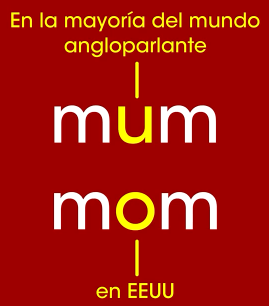
\includegraphics{2.png}
\end{figure}

La palabra ``mum'' en la gran mayoria de paises angloparlantes se escribe
con una u ya que lo hacen para mantener el sonido vocalico, lo que el
inglesito le llama sonido de cabernicola.

\begin{figure}[H]
\centering
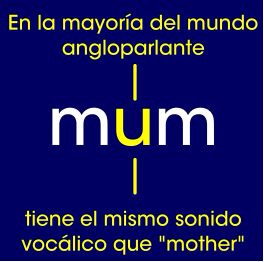
\includegraphics{3.png}
\end{figure}

Mientras que en estados unidos mantienen la o para tener coherencia con
la ortografia de mother.

\begin{figure}[H]
\centering
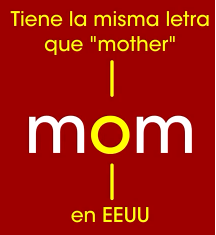
\includegraphics{4.png}
\end{figure}

Al final de las palabras father, mother, sister, brother. tienen el sonido
de cabernicola, es decir que no se han pronunciado la letra r.

\begin{figure}[H]
\centering
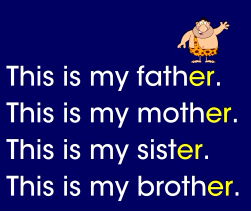
\includegraphics{5.png}
\end{figure}

very good!.

bye!.


